\documentclass[twoside,a4paper,12pt]{mwbk}

\usepackage[utf8]{inputenc}
%\usepackage{times}
\usepackage{amsmath,amssymb,amsthm}
\usepackage{xcolor}
\usepackage[final]{pdfpages}
\usepackage{graphicx}
%\usepackage[nottoc]{tocbibind}
\usepackage{caption}
\usepackage{subcaption}
\captionsetup{compatibility=false}
\usepackage{dsfont}
\usepackage{float}

\usepackage{booktabs}
\usepackage{array}


\setlength{\parindent}{0pt}

%\usepackage{geometry}
%\newgeometry{tmargin=2.5cm, bmargin=2.5cm, lmargin=2.5cm, rmargin=2.5cm}

%\numberwithin{equation}{section}
%\numberwithin{figure}{section}
\renewcommand{\thefigure}{\thechapter.\arabic{figure}}

%\newcommand*{\doi}[1]{\href{http://dx.doi.org/#1}{doi: #1}}
%\newcommand*{\MR}[1]{\href{http://www.ams.org/mathscinet-getitem?mr=#1&return=pdf}{MR #1}}
%\newcommand*{\ZBL}[1]{\href{http://www.zentralblatt-math.org/zmath/en/advanced/?q=an:#1&format=complete}{Zbl #1}}


\newcommand{\1}[1]{\mathds{1}\left(#1\right)}

\newenvironment{diagrams}[2]{\begin{figure}[p]
	%\centering
	\begin{subfigure}{.5\textwidth}
		\centering
		\includegraphics[width=\textwidth]{wykresy/#1.png}
		\caption{}
		\label{#1}
	\end{subfigure}
	\begin{subfigure}{.5\textwidth}
		\centering
		\includegraphics[width=\textwidth]{wykresy/#2.png}
		\caption{}
		\label{#2}
	\end{subfigure}
	}
	{
	\end{figure}
	}

\newenvironment{subdiagrams}[2]{
		\begin{subfigure}{.5\textwidth}
			\centering
			\includegraphics[width=\textwidth]{wykresy/#1.png}
			\caption{}
			\label{#1}
		\end{subfigure}
		\begin{subfigure}{.5\textwidth}
			\centering
			\includegraphics[width=\textwidth]{wykresy/#2.png}
			\caption{}
			\label{#2}
		\end{subfigure}
	} {}

\newenvironment{subdiagram}[1]{
	\begin{subfigure}{\textwidth}
		\centering
		\includegraphics[width=.9\textwidth]{wykresy/#1.png}
		\caption{}
		\label{#1}
	\end{subfigure}
} {}

\theoremstyle{plain}
\newtheorem{thm}{Theorem}[chapter]

\theoremstyle{definition}
\newtheorem{defn}[thm]{Definition}


\begin{document}
	
\begin{titlepage}
	
\includepdf{title_page.pdf}
\end{titlepage}


\tableofcontents

\chapter*{Introduction}

\textit{ ** Few words about my thesis...
Generally what is a data mining, what are the wavelets, what are the applications in data mining and finally, what is the main purpose - edge detection. **}

Data mining is connected with computing huge amount of data, thus to analyse those data it is require to use algorithms with low computational complexity. Wavelet transform is very efficient.


\textit{ ** VERY GOOD PARAGRAPH - JUST NEEDS TO BE WRITE WITH DIFFERENT WORDS **}
	
\textit{ Real world data sets are usually not directly suitable for performing Data
Mining algorithms. They contain noise, missing values and may be inconsistent.
In addition, real world data sets tend to be too large and high-dimensional.
Wavelets provide a way to estimate the underlying function from the data. With
the vanishing moment property of wavelets, we know that only some wavelet
coefficients are significant in most cases. By retaining selective wavelet coefficients,
wavelet transform could then be applied to denoising and dimensionality
reduction. Moreover, since wavelet coefficients are generally decorrelated,
we could transform the original data into wavelet domain and then carry out
Data Mining tasks.}

Pre-processing:

Denoising signals and images. Wavelet denoising - transform data into wavelet domain, remove noise components (with lower frequency) and then back to the original domain.

Data Transformation?

Dimensionality reduction. The idea is to simplify data, by getting rid off the less relevant information. In a wavelet domain we retain only the largest coefficients. Then, after getting back to the original domain we obtain simplified data.

Machine learning processing:

Clustering. Low frequency parts are correlated with regions of objects concentration and the high frequency parts correspond to the areas with sudden changes in the objects distribution. Thus, clustering can be conducted by recognising correlated components in the wavelet domain.

Classification.
Regression.
Distributed Data Mining.
Similarity Search/Indexing.
Approximate Query Processing.
Traffic Modelling.

\chapter{Wavelets theory}
A ''wavelet'' literally means a small wave. This term says a lot about its nature. Wavelets are a family of functions which oscillates like wave and should be compactly supported. Additionally, the wavelet has zero mean.

\begin{defn}
Wavelets are created by scaling and shifting of the, so called, mother wavelet $\psi(t)$. The child wavelets are defined as

\begin{equation}
\label{eq:wavelets}
\psi^{(a,b)}(t)=|a|^{-\frac{1}{2}} \psi\left(\frac{t-b}{a}\right),\ a>0,
\end{equation}

where $a$ is a scale parameter and $b$ translation parameter.

\end{defn}

There are plenty of different mother wavelets, for example

\begin{figure}[h]
	\centering
	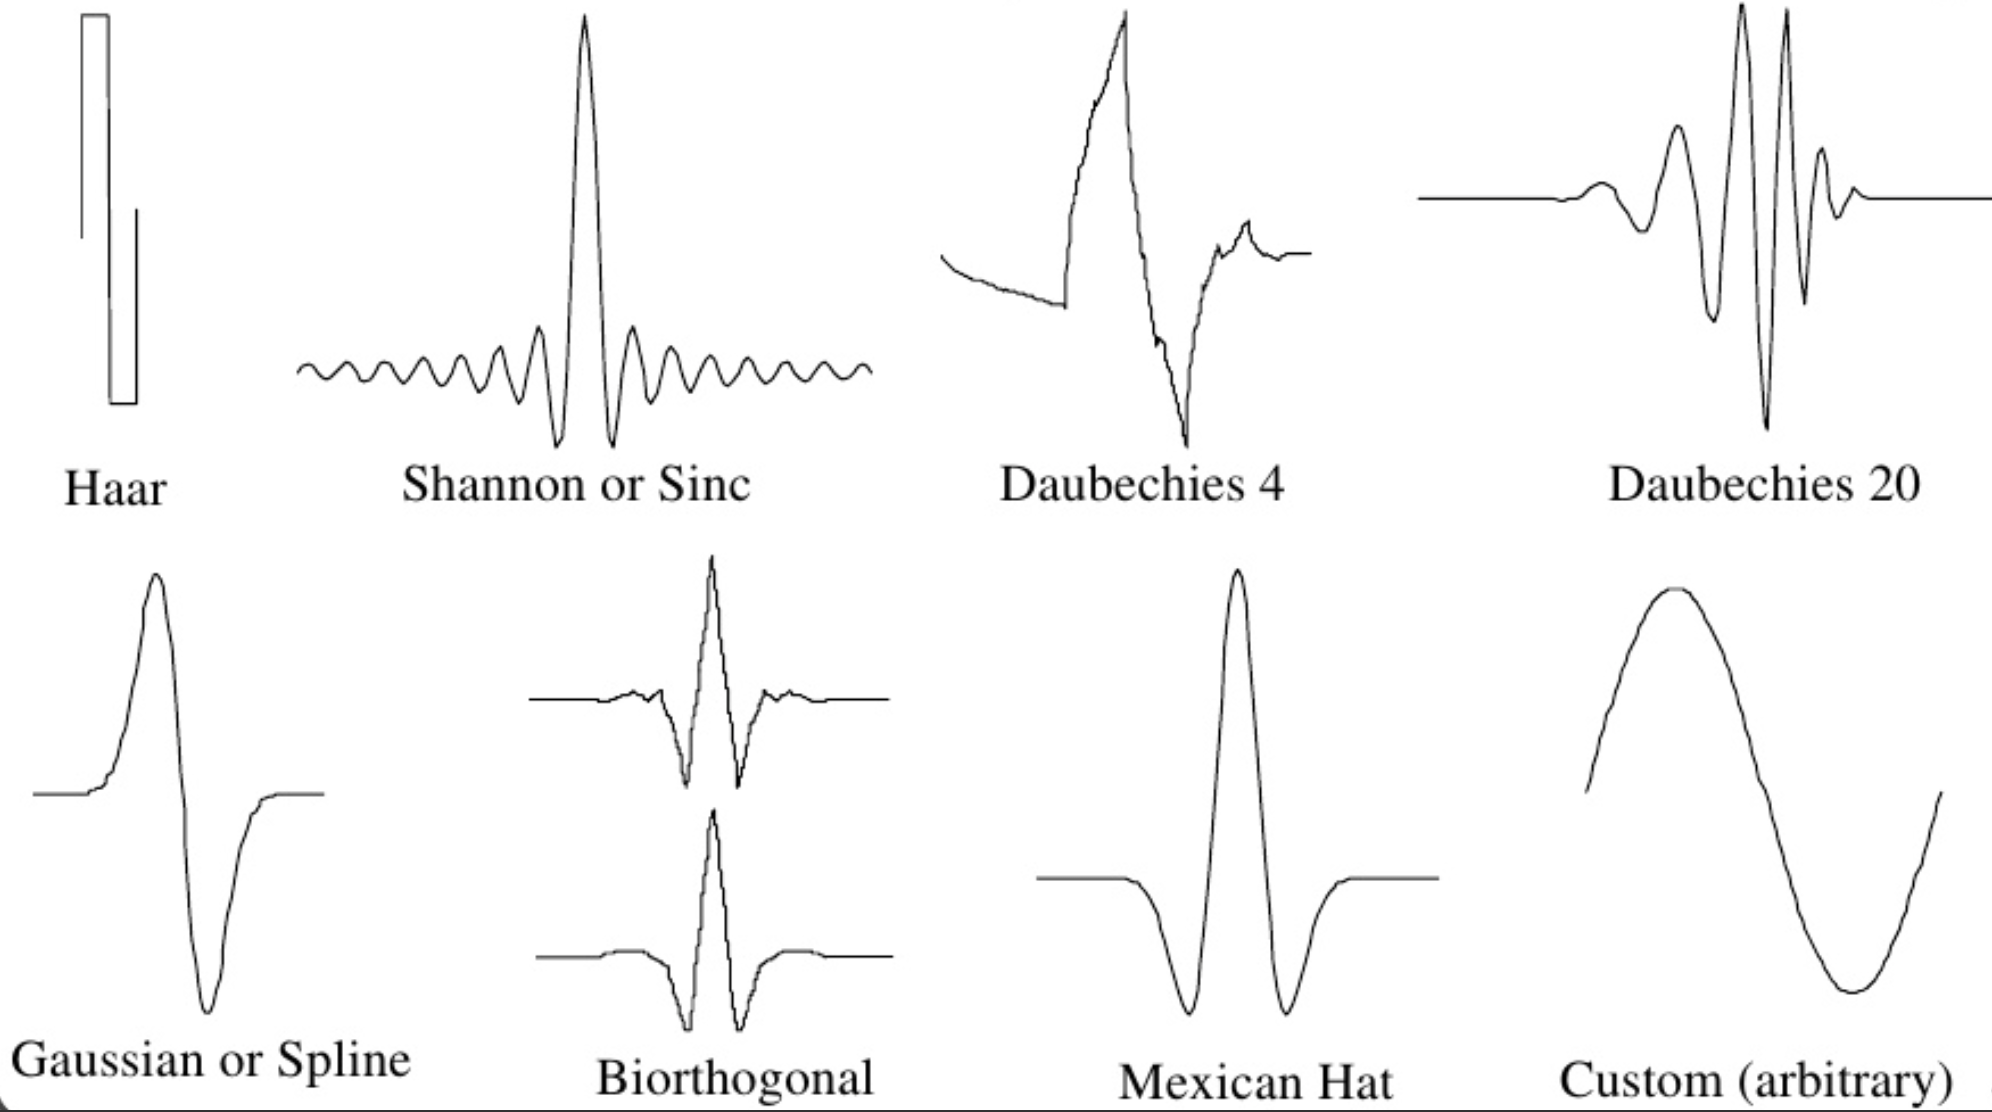
\includegraphics[width=\textwidth]{wavelets_with_bottom_line.png}
	\caption{Different types of wavelets.}
	\label{fig:wavelets}
\end{figure}

\textit{** Add more about wavelets properties! **}


\section{Daubechies wavelets}

Each type of wavelet function is more suitable for different applications. The best for image analysis are the Daubechies wavelets. 

\begin{defn}
Daubechies wavelets are collection of orthogonal and compactly supported functions. A denotation for those wavelets is $dbN$, where $N$ means a maximal number of vanishing moments.
\end{defn}

\begin{figure}[h]
	\centering
	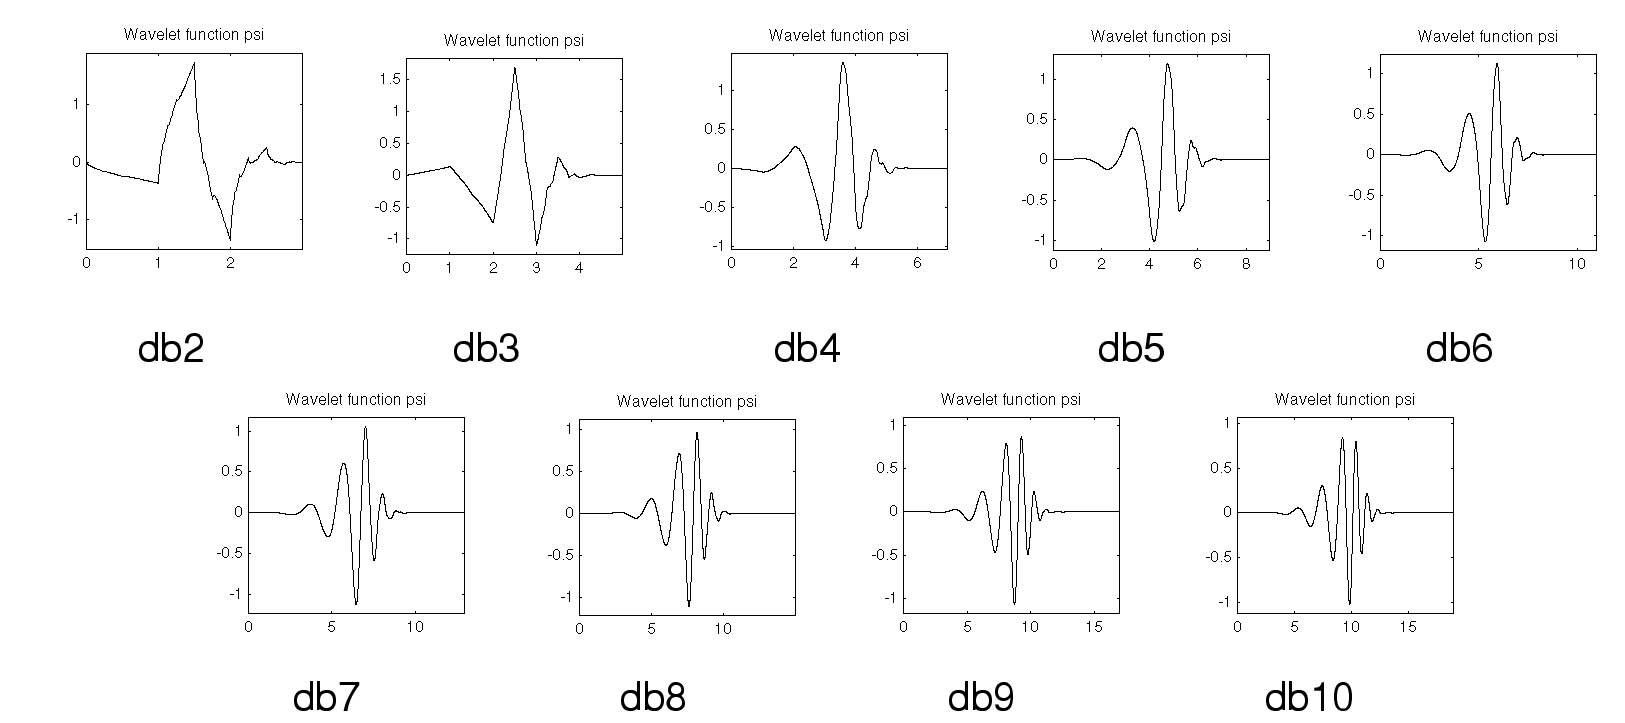
\includegraphics[width=\textwidth]{DB_N.png}
	\caption{Daubechies wavelets.}
	\label{fig:db_wavelets}
\end{figure}

\section{Wavelet Transform}

\textit{** Add some short introduction! -> po co to, co daje, do czego i dlaczego o tym piszemy  **}

\begin{defn}
Wavelet transform

\begin{equation}
W(a,b)=\int_{-\infty}^{\infty} y(t) a^{-\frac{1}{2}} \psi\left(\frac{t-b}{a}\right) dt,
\end{equation}

where $a$ is scale parameter, $b$ translation parameter and $y(t)$ original signal.
\end{defn}

\subsection{Wavelet transform vs Fourier transform}

\textit{** General information about integral transforms  **}

\begin{defn}
Fourier transform

\begin{equation}
Y(f)=\int_{-\infty}^{\infty} y(t) e^{-i\omega t} dt,
\end{equation}

where $y(t)$ is time domain signal and $Y(f)$ is frequency domain signal.
\end{defn}

\begin{table}[h]
\centering
\begin{tabular}{|p{0.5\linewidth}|p{0.5\linewidth}|}
\toprule
\textbf{ Wavelet transform} & \textbf{Fourier transform}
\\ \midrule
Suitable for stationary and non-\allowbreak -stationary signals 
& Suitable for stationary signals 
\\ \midrule
High time and frequency resolution
& Zero time resolution and very high frequency resolution     
\\ \midrule
Very suitable for studying the local behaviours of the signal
& No suitable  
\\ \midrule
Scaled and translated mother wavelets
& Sine and cosine waves
\\ \bottomrule
\end{tabular}
\caption{Differences between Wavelet Transform and Fourier Transform.}
\end{table}

What differs both transformations is the type of function. In Fourier case there are sine and cosine functions, wherein wavelet transform uses wavelets.

Why use the Wavelet transform?
Sine function oscillates on the whole real axis, thus it cannot represent abrupt changes. However, the Wavelet transform is localized in space and time, so it can be used to detect trends or sudden changes in signals and images. 

Moreover, wide range of wavelet functions is a main advantage of wavelet analysis.

\section{Discrete Wavelet transform}
There are two types of the wavelet transform:
\begin{itemize}
\item Continuous Wavelet Transform (CWT),
\item Discrete Wavelet Transform (DWT).
\end{itemize}

DWT is used to denoising and compression of signals and images. Also, DWT allows to detect smooth regions interrupted by edges or abrupt changes in contrast of images.

Scale and translation parameters are defined as

\begin{equation}
a = 2^j \text{ and } b = 2^j k,\ j,k=1,2,\ldots.
\end{equation}

to avoid redundancy in coefficients.


The figure \ref{fig:DWT} on a page \pageref{fig:DWT} shows how DWT works. Discrete Wavelet Transform splits signal with two filters: $g(n)$ - low pass filter (LPF) and $h(n)$ - high pass filter (HPF). The LPF captures a part with lower frequencies which refers to the main signal. Whereas, the HPF captures higher frequencies - a noise of the signal. Subsequently, both parts are downsampled by a factor of 2. This decomposition can be repeated on the LPF part of the signal. Hence, the next levels of DWT coefficients.

\begin{figure}[h]
	\centering
	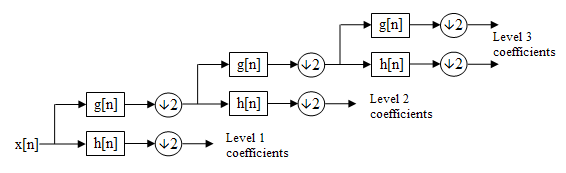
\includegraphics[width=\textwidth]{DWT.png}
	\caption{Discrete Wavelet transform on a signal $x(n)$.}
	\label{fig:DWT}
\end{figure}


\section{2-D Discrete Wavelet transform}
\label{sec:2D_DWT}

2-Dimensional Discrete Wavelet Transform works similar way as 1-D with High Pass Filter, Low Pass Filter and downsampling, except that one level of the decomposition includes double filtering, on columns and rows. The figure \ref{fig:2D_DWT} shows an image decomposition. Firstly, the DWT is applied on columns of the input image and then on the rows of the both outputs. Ultimately, there are four results:

\begin{itemize}
\item LL - result of LPF applied on both, columns and rows,
\item LH - result of LPF applied on columns and HPF on rows,
\item HL - result of HPF applied on columns and LPF on rows,
\item HH - result of HPF applied on both, columns and rows.
\end{itemize}  

\begin{figure}[h]
	\centering
	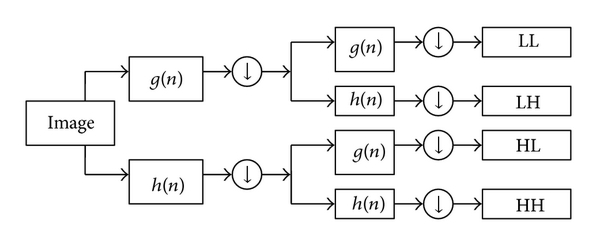
\includegraphics[width=\textwidth]{2D_DWT.JPG}
	\caption{2-D Discrete Wavelet transform on an image.}
	\label{fig:2D_DWT}
\end{figure}

Recall that the outcome of Low Pass Filter in the previous case was the main signal (without a noise). Thus, a 2-Dimensional equivalent is an approximation of an analysed image. The High Pass Filter captures high frequencies, then for an image the outcome are sudden changes in the image contrast. Now, lets focus on what exactly each result represent. First one, the LL is just an approximation of the initial image. Next, the LH shows abrupt changes in a horizontal direction, whereas the HL part presents similar issues but in a vertical direction. The HH shows sudden changes in a diagonal direction. In conclusion, the output of 2-D DWT gives us an approximation of the image and three parts with abrupt changes in different directions.

The Discrete Wavelet Transform has a wide range of applications in image processing, for example denoising, compressing 

\textit{** What are the possible applications of 2-D DWT - inne zastosowania w machine learning i data mining **}

What information gives us these sudden variations? Thanks to those we are able to find a places where two smooth regions meets. This kind of image anomaly could be interpreted as edges.

\section{Inverse Wavelet Transform}




\listoffigures
%\listoftables

%\bibliographystyle{unsrt} % w kolejności pojawienia
\bibliographystyle{abbrv} % w kolejności alfabetycznej
\bibliography{dokument_KK}
%\nocite{Buonaccorsi1987}
%\nocite{Edgeworth1918}
%\nocite{Wang2015}
	
\end{document}